\subsection{Measuring Master}

\subsubsection{Vorstellung}
\todo{Version, Downloaddatum, Playstore-Link}
Die App \mm{} von der Bosch GmbH ist im Play-Store unter der Rubrik ``Effizienz'' aufgelistet.
Selbst beschreibt der App-Hersteller seine Software wie folgt \citep{BoschMM}:

\begin{quote}
  ``Measuring Master ist eine multifunktionale App, die es ermöglicht, Aufmaße, Grundrisse und Temperaturmesswerte an einem Ort zu dokumentieren und zu verwalten.\\
  Die App ist besonders geeignet für Architekten, Maler, Bodenleger, Heizungsbauer und Elektriker, aber auch alle anderen Handwerker profitieren von der umfangreichen Funktionalität''
\end{quote}

\noindent
Nach dem Start der Applikation bietet sich die Möglichkeit ein neues Projekt anzulegen, oder bereits vorhandene Projekte zu bearbeiten.
Sobald das gewünschte Projekt ausgewählt wurde, kann der Benutzer durch das Ausklappen des Menüs an der linken Seite diverse Funktionen (siehe \autoref{fig:bmenu}) der App sehen. \\

\begin{figure}[h]
  \centering
  \begin{subfigure}[t]{0.4\textwidth}
    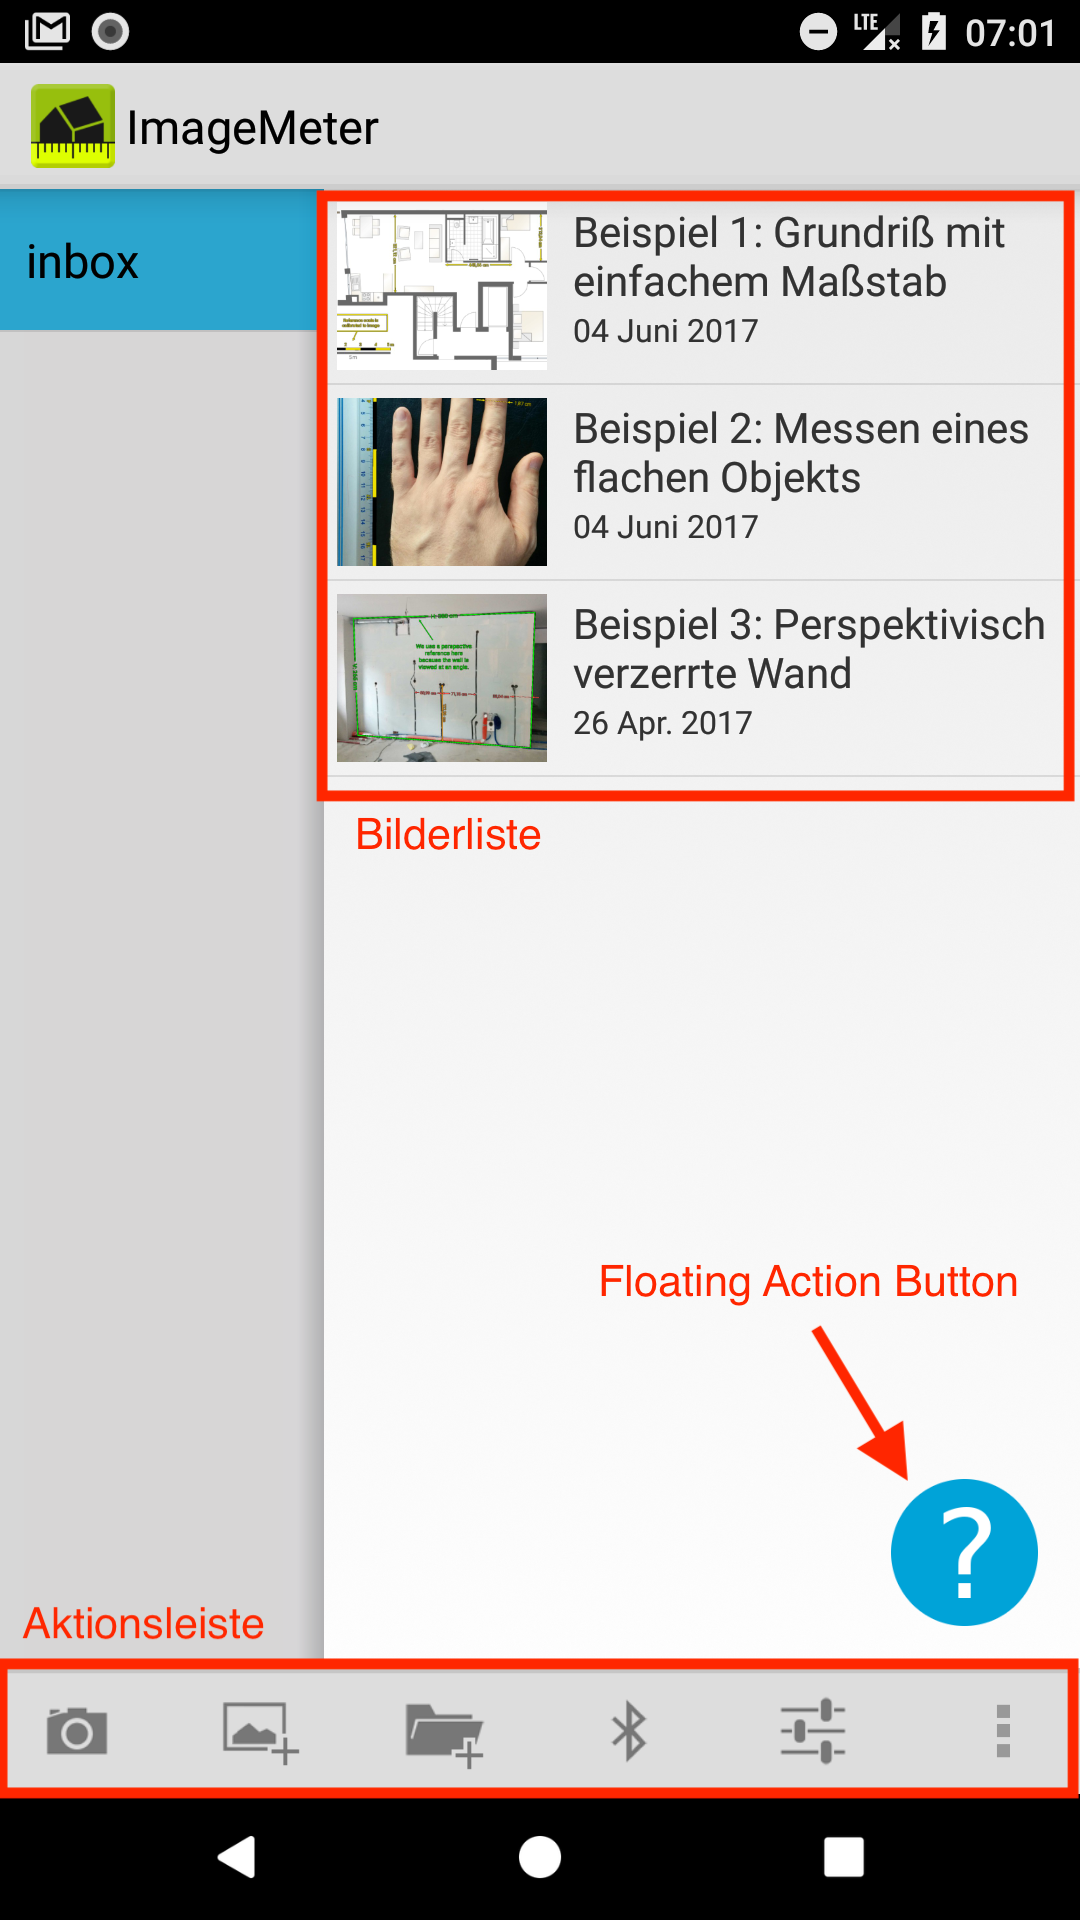
\includegraphics[keepaspectratio, width=\textwidth]{bosch/menu}
    \caption{Navigationsmenü}\label{fig:bmenu}	
  \end{subfigure}
  \begin{subfigure}[t]{0.4\textwidth}
    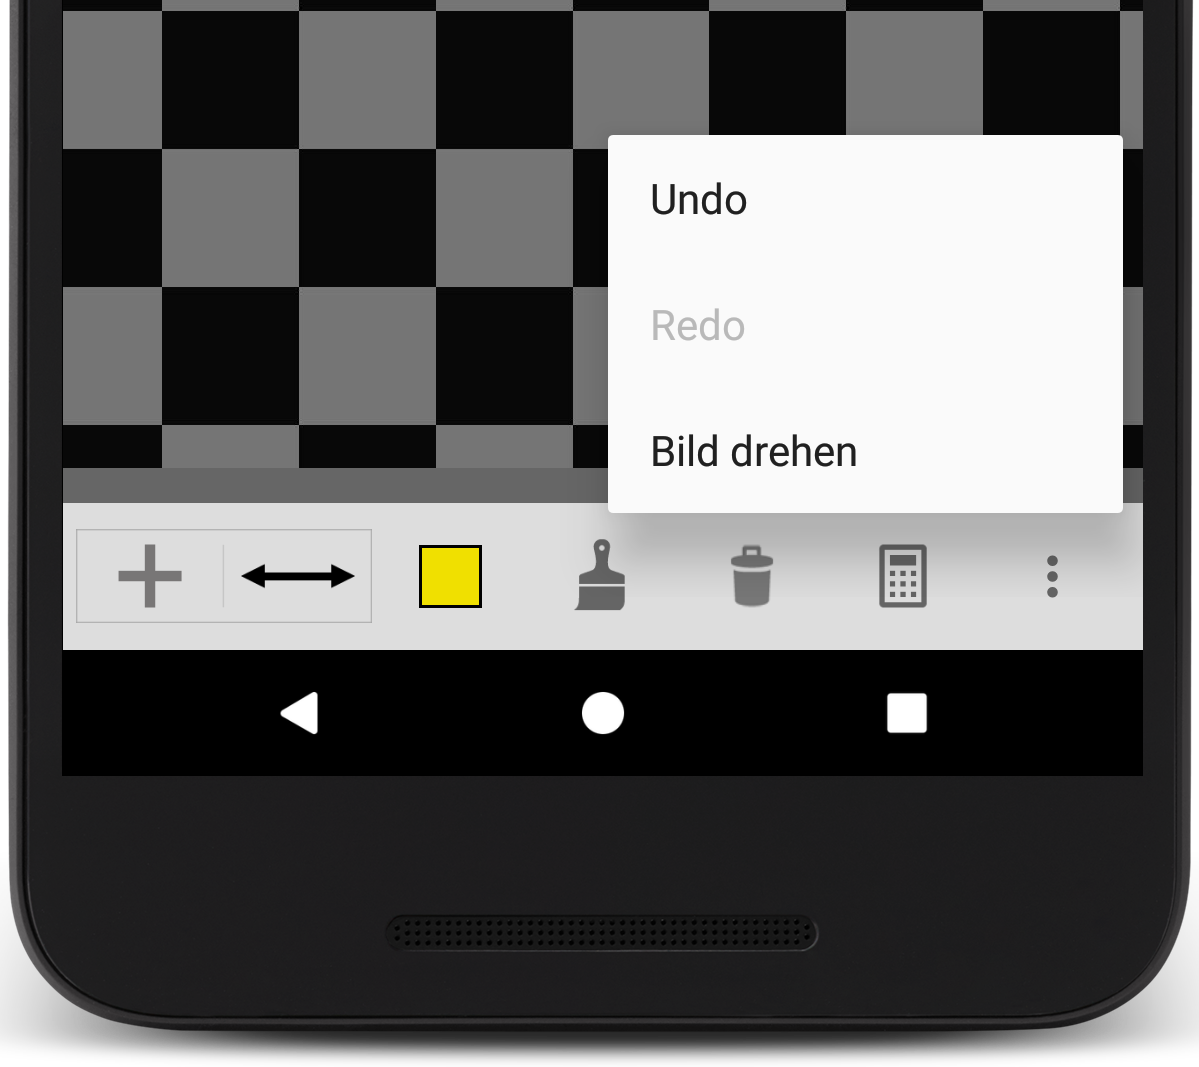
\includegraphics[keepaspectratio, width=\textwidth]{bosch/bar}
    \caption{Aufmaße-Funktion}\label{fig:bbar}
  \end{subfigure}
  \caption{\mm{} bei ausgeklapptem Navigationsmenü und in der Aufmaße-Funktion}
\end{figure}

Im Folgenden wird der Menüpunkt ``Aufmaße'' und die damit verbundene Funktionalität weiter vorgestellt und evaluiert.
So bietet sich dem Benutzer nach Auswahl der Aufmaße-Funktion die Möglichkeit, ausgewählte Bilder direkt mit Messwerten zu beschriften.
Hierzu können entweder Bilder direkt aus der Gallerie importiert, oder mit der Kamera aufgenommen werden.
Sobald der Benutzer den Foto-Import erfolgreich abgeschlossen hat, öffnet sich eine neue Ansicht, welche das ausgewählte Bild und weitere Bedienelement, in Form einer Statusleiste am unteren Rand, zeigt (siehe \autoref{fig:bbar}). \\

In dieser Benutzeroberfläche kann der Nutzer mit Hilfe von vier verschiedenen Formen (Linie, Viereck, Winkel, Freiform) Aufmaße ins Bild anzeichnen, und über einen Klick auf die gewünschte Form, Messwerte eintragen.
Außerdem bietet die App die Option, eine ausgewählte Reihe von Laserentfernungsmesser mit der App zu verbinden.
Dies ermöglicht eine Übertraung der gemessenen Distanzen über eine Bluetooth-Schnittstelle direkt an die App. \\

Um das annotierte Bild außerhalb der App weiter zu benutzen, bietet diese den Export als \emph{PDF} und \emph{JPEG} an.
Die exportierte \emph{PDF} enthält im Gegensatz zu der \emph{JPEG} zusätzlich zu dem annotierten Bild auch noch eine Tabelle mit allen eingetragenen Messwerten \autoref{fig:bexport}. 
Zudem lassen sich annotierte Bilder in der App speichern und zu einem späteren Zeitpunkt wieder bearbeiten.

\begin{figure}[h]
  \centering
  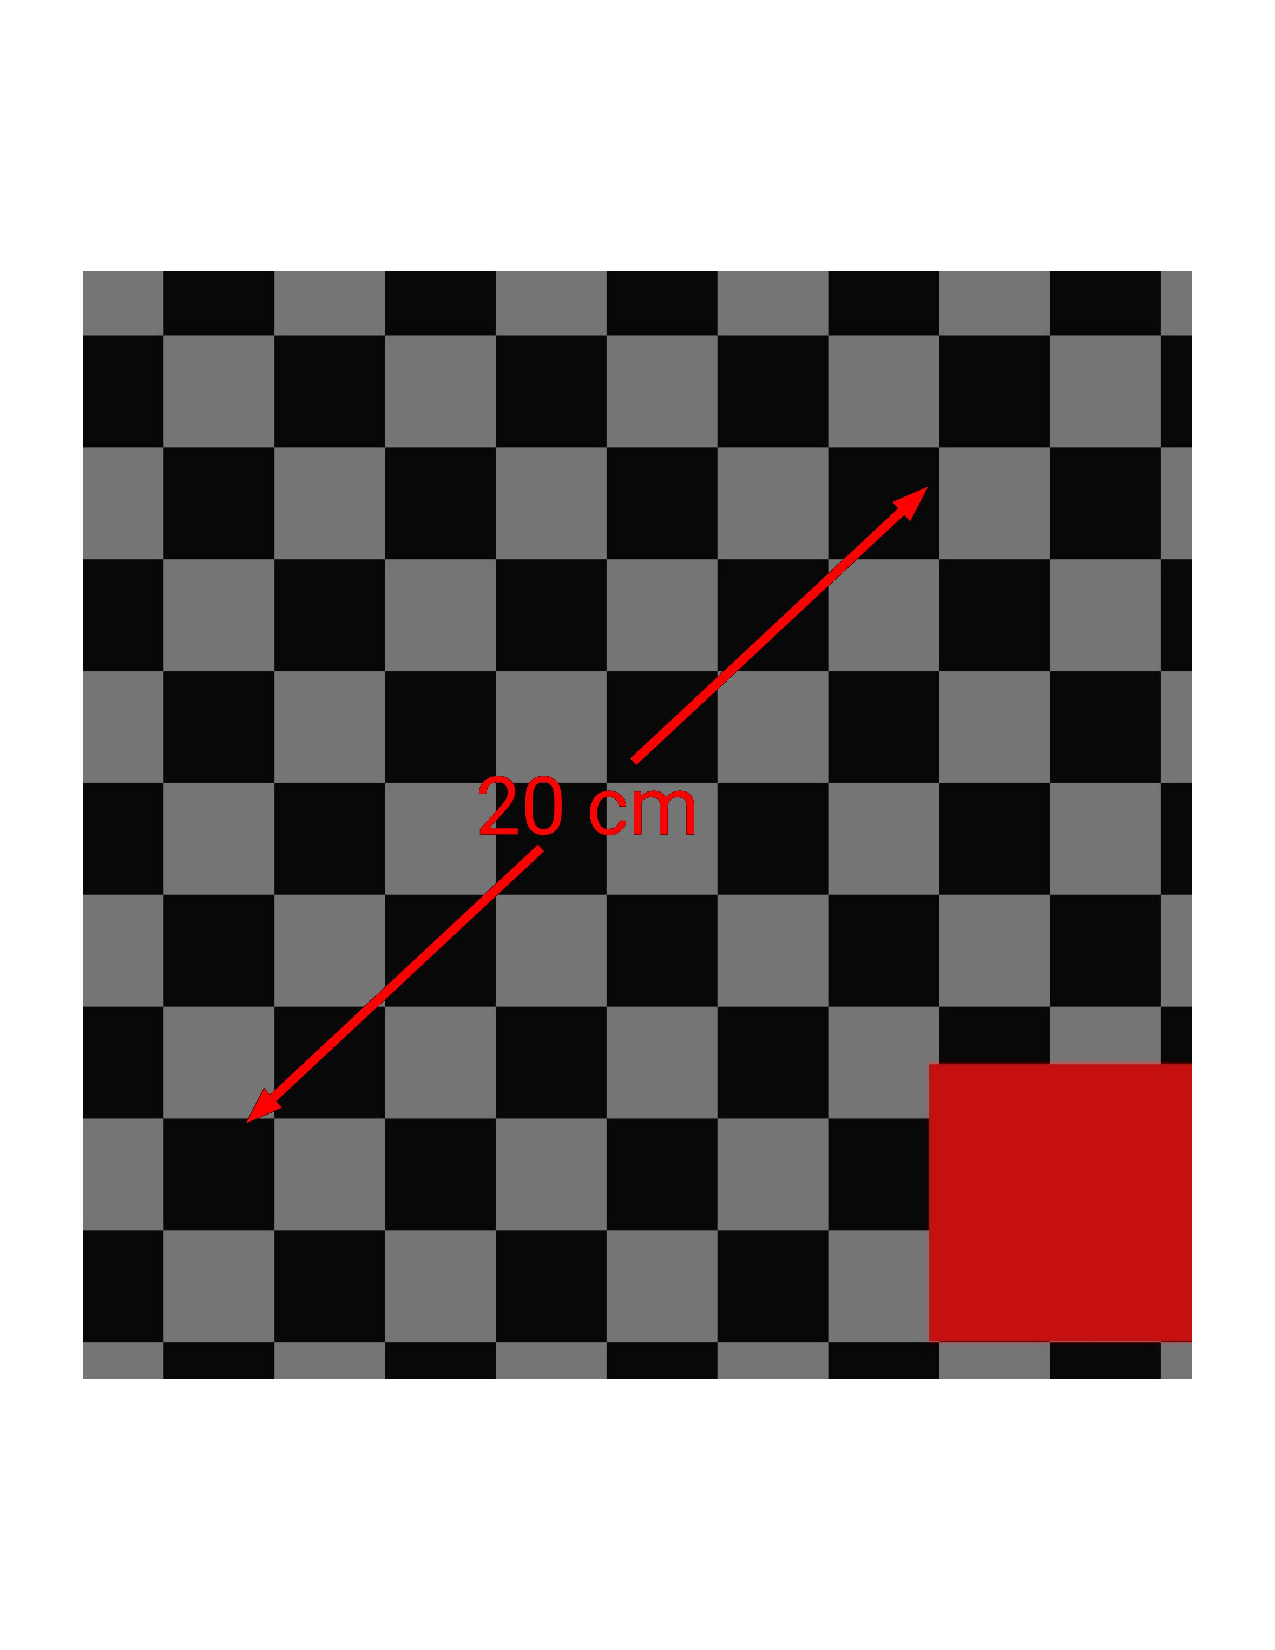
\includegraphics[keepaspectratio, width=\textwidth]{bosch/export}
  \caption{Exportierte PDF}\label{fig:bexport}
\end{figure}

\subsubsection{Evaluation}

Durch die Anzeige der Statusleiste am unteren Bildschirmrand (siehe \autoref{fig:bbar}) gibt die App dem Benutzer zu jeder Zeit eine klare und sichtbare Rückmeldung über den aktuellen Systemzustand (Nielsen~\autoref{itm:N1}). \\

Zusätzlich bietet ein erklärender Text im oberen Bereich des Bildschirms eine konkrete Hilfestellung zu den möglichen Aktionen, die der Benutzer im aktuellen Systemzustand ausführen kann (Nielsen~\autoref{itm:N10}). \\

Darüber hinaus kann der Nutzer über ein Undo- bzw. Redo-Symbol fehlerhafte oder unabsichtliche Eingaben rückgängig machen, oder rückgängig gemachte Aktionen wiederholen (Nielsen~\autoref{itm:N3}).
Dadurch, dass Aktionen nur dann ausführbar sind, wenn man den richtigen Modus in der Statusleiste ausgewählt hat, werden Fehler präventiv vermieden (siehe \autoref{fig:bicons}).
So lassen sich Formen erst dann löschen, wenn diese zuvor markiert wurde, oder Aktionen rückgängig machen, wenn zuvor eine Benutzeraktion stattgefunden hat (Nielsen~\autoref{itm:N5}). \\

\begin{figure}[h]
  \centering
  
\includegraphics[keepaspectratio, width=\textwidth]{bosch/icons}
  \caption{Menüleiste bei ausgewählter Form und vorheriger Zeichen-Aktion}
  \label{fig:bicons}
\end{figure}

Schafft man es trotzdem einen Fehlerzustand des Systems herzustellen, wird dieser durch einen ``Toast'' \todo{def} erkennbar gemacht, und gibt dem Benutzer Feedback darüber, was zum Fehler geführt hat \todo{Bild vom Toast beim Bildimport} (Nielsen~\autoref{itm:N9}). \\

Durch die konsistente Benutzung bekannter Icons lassen sich die dahinter befindlichen Aktionen intuitiv erkennen, und die Gedächtnislast des Benutzers reduzieren. 
So wird zum Beispiel sowohl im ``Zeichen-'' als auch im ``Text-Modus'' das Mülleimer-Icon (siehe \autoref{fig:bicons}) in der oberen Statusleiste als Löschfunktion der markierten Form bzw.\ des ausgewählten Textes benutzt (Nielsen~\autoref{itm:N4} \& \autoref{itm:N6}). \\

Einen ``Expertenmodus'', der dem Benutzer voreingestelle Aktionen ändern, oder Abkürzungen für bestimmte Schritte nehmen lässt, gibt es in dieser App nicht (Nielsen~\autoref{itm:N7}).
So muss der Nutzer jedesmal, wenn er ein eine zuvor eingezeichnete Form beschriften will, in den ``Text-Modus'' wechseln, die gewünschte Form markieren, und anschließend die Messwerte eintragen. 
Alternativ hätte man hier zum Beispiel die Benutzung einer langen Klick-Aktion auf die gewünschte Form zum Beschrfiten nutzen können. \\

Durch das Hervorheben der markierten Form durch eine andere Farbe ermöglicht die App ein schnelles und effizientes Scannen des Bildschirminhaltes (Nielsen~\autoref{itm:N12}). \\

Das Malen von Formen durch das Klicken und anschließende Ziehen mit einem Finger auf dem Bildschirm ermöglicht eine einfache und effiziente Benutzung mit einer Hand (Nielsen~\autoref{itm:N17}).
Zusätzlich wird mit Hilfe einer Lupe, die sich beim Zeichnen stets neben dem Finger befindet, der Bereich unter dem Finger vergößert dargestellt (siehe \autoref{fig:blense}).
Dies macht das Malen von Formen nicht nur effizienter, sondern beugt auch Fehlern vor, da dieser Bereich sonst vom Finger des Benutzer bedeckt ist und man nicht sehen würde, wo genau man malt. \\

\begin{wrapfigure}{R}{0.5\textwidth}
  \centering
  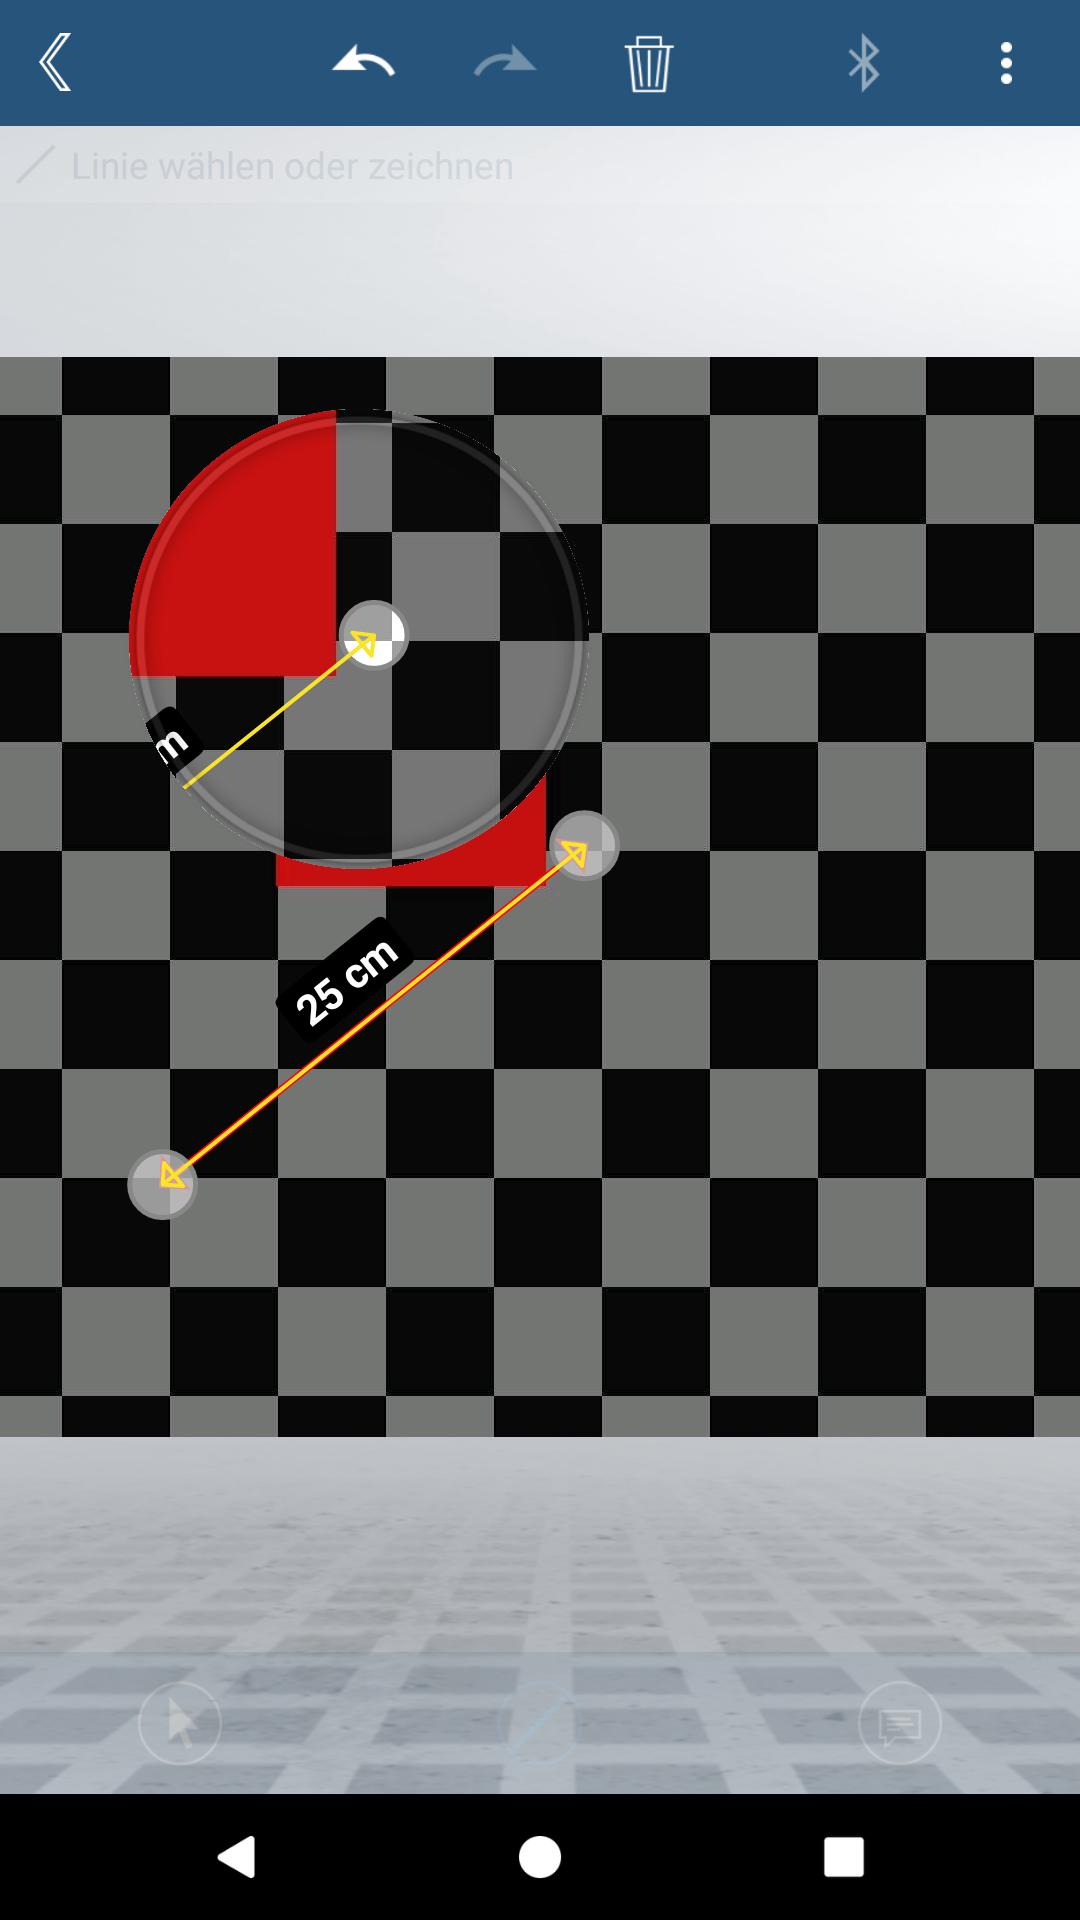
\includegraphics[keepaspectratio, width=0.5\textwidth]{bosch/lense}
  \caption{Zoom-Linse beim Zeichnen einer Form}
  \label{fig:blense}
\end{wrapfigure}

Des Weiteren kann die App zu jeder Zeit pausiert werden, ohne dass eingetragene Messwerte oder Formen verloren gehen (Nielsen~\autoref{itm:N11}). \\

Im Kontrast dazu führen Bildschirmrotationen vom Hoch- ins Querformat zu einer verwirrenden Drehung des Bildes, welches sich entgegen aller Erwartungen mit der Bildschirmausrichtung dreht, und nicht in der Ausrichtung, in der es aufgenommen wurde bleibt (Nielsen~\autoref{itm:N15}). \\

Zudem führt die teilweise fehlerhafte Umsetzung der Gesten-Unterstützung dazu, dass der Nutzer beim Zoomen des Bildes unabsichtlich eine Form malt, wenn er zuvor im ``Zeichen-Modus'' ist (Nielsen~\autoref{itm:N16}).
Dieser Punkt schmälert eine positive Benutzerfahrung enorm, da dies nach fast jeder Zoom-Aktion eine Undo-Aktion erzwingt, um die unabsichtlich-gemalte Form wieder zu entfernen (Nielsen~\autoref{itm:N13}). \\

Der Export des bearbeiteten Bildes führt dazu, dass alle eingetragenen Messwerte nicht mehr trivial auslesbar sind (da nicht als Meta-Daten verfügbar). Zudem würde sich die App nur schwer in eine bestehende Systemarchitektur integrieren lassen, da der Punkt der Aufmaßerfassung nur eine von vielen Funktionen der App ist. \todo{ref auf weitere Kriterien} \\

Zusammenfassend lässt sich also festhalten, dass die App \mm{} von der Bosch GmbH die Heuristiken nach Nielsen größtenteils erfüllt, sich jedoch Mängel bei der Benutzung von Gesten zum Zoomen im Bild und der Unterstützung von verschiedenen Bildschirmausrichtungen identifizieren lassen haben.
Dies sind Punkte, welche nicht nur eine positive Nutzungserfahrung schmälern, sondern auch potentielle Fehlerquellen, die durch die Benutzung einer Android-App minimiert werden sollten, vergößern.
Zudem lässt sich die Aufmaß-Funktion nicht in die bestehende Android-App integrieren, da es keine Möglichkeit gibt, annotierte Bilder inklusive der Meta-Daten an eine andere App zu teilen bzw. in einer anderen App aufgenommene Bilder direkt an \mm{} freizugeben.
Auch die eingetragenen Messwerte lassen sich im Nachhinein nur mühsam aus dem Bild extrahieren, da diese nicht mehr als Meta-Daten vorliegen, sodass die Weiterverarbeitung in einem nachgeschalteten Dienst wie einer \emph{API} nicht möglich sind.
